
%%%%%%%%%%%%%%%%%%%%%%% file typeinst.tex %%%%%%%%%%%%%%%%%%%%%%%%%
%
% This is the LaTeX source for the instructions to authors using
% the LaTeX document class 'llncs.cls' for contributions to
% the Lecture Notes in Computer Sciences series.
% http://www.springer.com/lncs       Springer Heidelberg 2006/05/04
%
% It may be used as a template for your own input copy it
% to a new file with a new name and use it as the basis
% for your article.
%
% NB: the document class 'llncs' has its own and detailed documentation, see
% ftp://ftp.springer.de/data/pubftp/pub/tex/latex/llncs/latex2e/llncsdoc.pdf
%
%%%%%%%%%%%%%%%%%%%%%%%%%%%%%%%%%%%%%%%%%%%%%%%%%%%%%%%%%%%%%%%%%%%


\documentclass[runningheads,a4paper]{llncs}

\usepackage{amssymb}
\setcounter{tocdepth}{3}
\usepackage{graphicx}

\usepackage{url}

\begin{document}

\mainmatter  % start of an individual contribution

% first the title is needed
\title{Big Data Platform}

% a short form should be given in case it is too long for the running head
\titlerunning{Big Data Platform}

% the name(s) of the author(s) follow(s) next
%
% NB: Chinese authors should write their first names(s) in front of
% their surnames. This ensures that the names appear correctly in
% the running heads and the author index.
%
\author{
Sung-Soo Kim, Jongho Won
}

%
%\authorrunning{Lecture Notes in Computer Science: Authors' Instructions}
% (feature abused for this document to repeat the title also on left hand pages)

% the affiliations are given next; don't give your e-mail address
% unless you accept that it will be published
\institute{ETRI\\
218 Gajeong-ro, Yuseong-gu, Deajeon, South Korea\\
\url{{sungsoo, jhwon}@etri.re.kr}\\
\url{http://www.etri.re.kr}}

%
% NB: a more complex sample for affiliations and the mapping to the
% corresponding authors can be found in the file "llncs.dem"
% (search for the string "\mainmatter" where a contribution starts).
% "llncs.dem" accompanies the document class "llncs.cls".
%

\toctitle{Lecture Notes in Computer Science}
\tocauthor{Authors' Instructions}
\maketitle


\begin{abstract}
Recent advances of software defined networking and optical switching technology make it possible to program the network stack all the way from physical topology to flow level traffic control. In this paper, we leverage the combination of SDN controller with optical switching to explore the tight integration of application and network control. We particularly study the run-time network configuration for big data applications to jointly optimize application performance and network utilization. We use Hadoop as an example to discuss the integrated network control architecture, job scheduling, topology and routing configuration mechanisms for Hadoop jobs. Our analysis suggests that such an integrated control has great potential to improve application performance with relatively small configuration overhead. We believe our study shows early promise of achieving the long-term goal of tight network and application integration using SDN.
\keywords{We would like to encourage you to list your keywords within
the abstract section}
\end{abstract}


\section{Introduction}
Network engineers and researchers have long sought effective ways to make networks more “application-aware”. A variety of methods for optimizing the network to improve application per- formance or availability have been considered. Some of these ap- proaches have been edge-based, for example tuning protocol pa- rameters at end-hosts to improve throughput [28], or choosing over- lay nodes to direct traffic over application-optimized paths [23]. Examples of network-centric approaches include providing custom instances of routing protocols to applications [10], or even allowing applications to embed code in network devices to perform applica- tion processing [24].

While these earlier efforts have met with varying degrees of suc- cess and adoption, the recent emergence of the software-defined networking paradigm has created renewed interest in tailoring the network to better meet the needs of applications. By providing a well-defined programming interface to the network (e.g., Open- Flow), SDN provides an opportunity for more dynamic and flexi- ble interaction with the network. Despite this promising vision, the ability of SDN to effectively configure or optimize the network to improve application performance and availability is still nascent.
Recently, two concomitant trends in data center applications and network architecture present a new opportunity to leverage the ca- pabilities of SDN for truly application-aware networking. The first is the growing prominence of big data applications which are used to extract value and insights efficiently from very large volumes of data [1, 2, 20, 29]. Many of these applications process data ac- cording to well-defined computation patterns, and also have a cen- tralized management structure which makes it possible to leverage application-level information to optimize the network. The second trend is the growing number of proposals for data center network architectures that leverage optical switches to provide significantly increased point-to-point bandwidth with low cabling complexity and energy consumption [26, 18, 15, 25]. Some of this work has demonstrated how to collect network-level traffic data and intelli- gently allocate optical circuits between endpoints (e.g., top-of-rack switches) to improve application performance. But without a true application-level view of traffic demands and dependencies, circuit utilization and application performance can be poor [14].
These three trends taken together – software-defined networking, dynamically reconfigurable optical circuits, and structured big data applications – motivate us to explore the design of an SDN con- troller using a “cross-layer” approach that configures the network based on big data application dynamics at run-time. In this paper, we focus on Hadoop as an example to explore the design of an inte- grated network control plane, and describe Hadoop job scheduling strategies to accommodate dynamic network configuration. We in- troduce the topology construction and routing mechanisms for a number of communication patterns, including single aggregation, data shuffling, and partially overlapping aggregation traffic patterns to improve application performance.
The proposed topology configuration algorithms can be imple- mented using a small number of OpenFlow rules on each switch. Our preliminary estimation suggests that the flow rule installation introduces low overhead compared to the relatively long duration of MapReduce jobs. However, a number of challenges remain which have implications for SDN controller architectures. For example, in contrast to common SDN use cases such as WAN traffic engi- neering [12] and cloud network provisioning [8], run-time network configuration for big data jobs requires more rapid and frequentflow table updates. This imposes significant requirements on the scalability of the SDN controller and how fast it can update state across the network. Another challenge is in maintaining consistent network-wide routing updates with low latency, and in coordinat- ing network reconfiguration requests from different applications in multi-tenancy environments.
This is a work-in-progress, and there is clearly more work to be done to realize and fully evaluate the design. Nevertheless, we be- lieve that this work shows early promise for achieving one of the oft-cited goals of software-define networking, that is to tightly in- tegrate applications with the network to improve performance and utilization.

\section{INTEGRATED NETWORK CONTROL ARCHITECTURE}
In this section, we describe the overall architecture of cross-layer network control for big data applications.

\subsection{System Architecture}
Figure 1 shows the system architecture of a cross-layer network control plane. We assume a hybrid electrical and optical data cen- ter network where OpenFlow-enabled top-of-rack (ToR) switches are connected to two aggregation networks, a multi-root tree with Ethernet switches and a MEMS-based optical circuit switch1. Each ToR switch has multiple optical uplinks connected to the optical switch (commodity switches typically have 4 to 6 uplinks). All the switches are controlled by a SDN controller which manages physical connectivity among ToR switches over optical circuits by configuring the optical switch. It can also manage the forwarding at ToR switches using OpenFlow rules.
Many big data applications, such as Hadoop [1], Dryad [20], Spark [29] and HBase [2], have a master node, or application con- troller, that manages all incoming job requests. To support cross- layer network control, the SDN controller is interfaced to the mas- ter node for each individual application, such as the Hadoop sched- uler or HBase master. It could also connect to broader coordination frameworks such as Mesos [13] that manage multiple co-existing applications sharing the data center.
Since the SDN controller may be shared among multiple applica- tions, it provides a general interface to configure devices and con- trol forwarding in the network. It also provides a query interface to make authoritative network information available to applications. For big data applications, the SDN controller provides an interface that accepts traffic demand matrices from application controllers in a standard format. The traffic demand matrix describes the vol-ume and policy requirements for traffic exchanged between differ- ent source and destination racks.
Using the network configuration interface, application controllers report traffic demands and structure from one or multiple jobs and issue a network configuration command to set up the topology ac- cordingly. They can also use network information provided by the SDN controller, such as topology, to make more informed decisions on job scheduling and placement (further described in Section 3.2). Application controllers implement their own application-specific mechanisms to collect traffic demands from different components, and also define appropriate criteria to correlate and aggregate de- mands from multiple jobs.

\subsection{Traffic Pattern of Big Data Applications}

The traffic in big data applications consists of bulk transfer, data aggregation/partitioning, and latency sensitive control messages. The control traffic is typically low data rate and can be handled eas- ily by even a relatively slow Ethernet. In our architecture, control messages are always sent over the packet switched network using default routes that direct traffic over the Ethernet2.
Data aggregation and partitioning, where data are partitioned or aggregated between one server and a large number of other servers, is a common traffic pattern. For example, in MapReduce, the inter- mediate results from all the mappers will be aggregated at a reducer for performing the reduce function. The shuffle phase of MapRe- duce is actually a combination of multiple data aggregation patterns between mappers and reducers. In parallel database systems, most operations require merging and splitting data from different tables. Data aggregation requires high bandwidth to exchange large vol- umes of data between a potentially large number of servers. In the typical case of oversubscribed data center networks, the data aggre- gation and shuffling patterns can easily become performance bot- tlenecks. Our cross-layer network controller is designed primarily to address the challenge of handling a mix of multiple aggregation and data shuffling tasks.

\subsection{The Advantage of Application Awareness}
For big data applications, an application-aware network controller provides improved performance. By carefully allocating and schedul- ing high-bandwidth links via optical paths, job completion time can be reduced significantly. Data center operators also benefit from better utilization of the relatively limited set of high-bandwidth op- tical links.
Current approaches for allocating optical circuits in data centers, such as c-Through [26], Helios [18] and OSA [15], rely on network level statistics to estimate the traffic demand matrix in the data cen- ter. While these designs show the potential to benefit applications, recent work has shown that without a true application-level view of traffic demands and dependencies, circuit utilization and applica- tion performance can be poor [14]. First, it is difficult to estimate real application traffic demand based only on readings of network level statistics. Without accurate information about application de- mand, optical circuits may be configured between the wrong lo- cations, or circuit flapping may occur from repeated corrections. Second, blindly optimizing circuit throughput without considering application structure could cause blocking among interdependent applications and poor application performance.

\end{document}


%You are strongly encouraged to use \LaTeXe{} for the
%preparation of your camera-ready manuscript together with the
%corresponding Springer class file \verb+llncs.cls+. Only if you use
%\LaTeXe{} can hyperlinks be generated in the online version
%of your manuscript.
%
%The \LaTeX{} source of this instruction file for \LaTeX{} users may be
%used as a template. This is
%located in the ``authors'' subdirectory in
%\url{ftp://ftp.springer.de/pub/tex/latex/llncs/latex2e/instruct/} and
%entitled \texttt{typeinst.tex}. There is a separate package for Word 
%users. Kindly send the final and checked source
%and PDF files of your paper to the Contact Volume Editor. This is
%usually one of the organizers of the conference. You should make sure
%that the \LaTeX{} and the PDF files are identical and correct and that
%only one version of your paper is sent. It is not possible to update
%files at a later stage. Please note that we do not need the printed
%paper.
%
%We would like to draw your attention to the fact that it is not possible
%to modify a paper in any way, once it has been published. This applies
%to both the printed book and the online version of the publication.
%Every detail, including the order of the names of the authors, should
%be checked before the paper is sent to the Volume Editors.
%
%\subsection{Checking the PDF File}
%
%Kindly assure that the Contact Volume Editor is given the name and email
%address of the contact author for your paper. The Contact Volume Editor
%uses these details to compile a list for our production department at
%SPS in India. Once the files have been worked upon, SPS sends a copy of
%the final pdf of each paper to its contact author. The contact author is
%asked to check through the final pdf to make sure that no errors have
%crept in during the transfer or preparation of the files. This should
%not be seen as an opportunity to update or copyedit the papers, which is
%not possible due to time constraints. Only errors introduced during the
%preparation of the files will be corrected.
%
%This round of checking takes place about two weeks after the files have
%been sent to the Editorial by the Contact Volume Editor, i.e., roughly
%seven weeks before the start of the conference for conference
%proceedings, or seven weeks before the volume leaves the printer's, for
%post-proceedings. If SPS does not receive a reply from a particular
%contact author, within the timeframe given, then it is presumed that the
%author has found no errors in the paper. The tight publication schedule
%of LNCS does not allow SPS to send reminders or search for alternative
%email addresses on the Internet.
%
%In some cases, it is the Contact Volume Editor that checks all the final
%pdfs. In such cases, the authors are not involved in the checking phase.
%
%\subsection{Additional Information Required by the Volume Editor}
%
%If you have more than one surname, please make sure that the Volume Editor
%knows how you are to be listed in the author index.
%
%\subsection{Copyright Forms}
%
%The copyright form may be downloaded from the ``For Authors"
%(Information for LNCS Authors) section of the LNCS Website:
%\texttt{www.springer.com/lncs}. Please send your signed copyright form
%to the Contact Volume Editor, either as a scanned pdf or by fax or by
%courier. One author may sign on behalf of all of the other authors of a
%particular paper. Digital signatures are acceptable.
%
%\section{Paper Preparation}
%
%Springer provides you with a complete integrated \LaTeX{} document class
%(\texttt{llncs.cls}) for multi-author books such as those in the LNCS
%series. Papers not complying with the LNCS style will be reformatted.
%This can lead to an increase in the overall number of pages. We would
%therefore urge you not to squash your paper.
%
%Please always cancel any superfluous definitions that are
%not actually used in your text. If you do not, these may conflict with
%the definitions of the macro package, causing changes in the structure
%of the text and leading to numerous mistakes in the proofs.
%
%If you wonder what \LaTeX{} is and where it can be obtained, see the
%``\textit{LaTeX project site}'' (\url{http://www.latex-project.org})
%and especially the webpage ``\textit{How to get it}''
%(\url{http://www.latex-project.org/ftp.html}) respectively.
%
%When you use \LaTeX\ together with our document class file,
%\texttt{llncs.cls},
%your text is typeset automatically in Computer Modern Roman (CM) fonts.
%Please do
%\emph{not} change the preset fonts. If you have to use fonts other
%than the preset fonts, kindly submit these with your files.
%
%Please use the commands \verb+\label+ and \verb+\ref+ for
%cross-references and the commands \verb+\bibitem+ and \verb+\cite+ for
%references to the bibliography, to enable us to create hyperlinks at
%these places.
%
%For preparing your figures electronically and integrating them into
%your source file we recommend using the standard \LaTeX{} \verb+graphics+ or
%\verb+graphicx+ package. These provide the \verb+\includegraphics+ command.
%In general, please refrain from using the \verb+\special+ command.
%
%Remember to submit any further style files and
%fonts you have used together with your source files.
%
%\subsubsection{Headings.}
%
%Headings should be capitalized
%(i.e., nouns, verbs, and all other words
%except articles, prepositions, and conjunctions should be set with an
%initial capital) and should,
%with the exception of the title, be aligned to the left.
%Words joined by a hyphen are subject to a special rule. If the first
%word can stand alone, the second word should be capitalized.
%
%Here are some examples of headings: ``Criteria to Disprove
%Context-Freeness of Collage Language", ``On Correcting the Intrusion of
%Tracing Non-deterministic Programs by Software", ``A User-Friendly and
%Extendable Data Distribution System", ``Multi-flip Networks:
%Parallelizing GenSAT", ``Self-determinations of Man".
%
%\subsubsection{Lemmas, Propositions, and Theorems.}
%
%The numbers accorded to lemmas, propositions, and theorems, etc. should
%appear in consecutive order, starting with Lemma 1, and not, for
%example, with Lemma 11.
%
%\subsection{Figures}
%
%For \LaTeX\ users, we recommend using the \emph{graphics} or \emph{graphicx}
%package and the \verb+\includegraphics+ command.
%
%Please check that the lines in line drawings are not
%interrupted and are of a constant width. Grids and details within the
%figures must be clearly legible and may not be written one on top of
%the other. Line drawings should have a resolution of at least 800 dpi
%(preferably 1200 dpi). The lettering in figures should have a height of
%2~mm (10-point type). Figures should be numbered and should have a
%caption which should always be positioned \emph{under} the figures, in
%contrast to the caption belonging to a table, which should always appear
%\emph{above} the table; this is simply achieved as matter of sequence in
%your source.
%
%Please center the figures or your tabular material by using the \verb+\centering+
%declaration. Short captions are centered by default between the margins
%and typeset in 9-point type (Fig.~\ref{fig:example} shows an example).
%The distance between text and figure is preset to be about 8~mm, the
%distance between figure and caption about 6~mm.
%
%To ensure that the reproduction of your illustrations is of a reasonable
%quality, we advise against the use of shading. The contrast should be as
%pronounced as possible.
%
%If screenshots are necessary, please make sure that you are happy with
%the print quality before you send the files.
%\begin{figure}
%\centering
%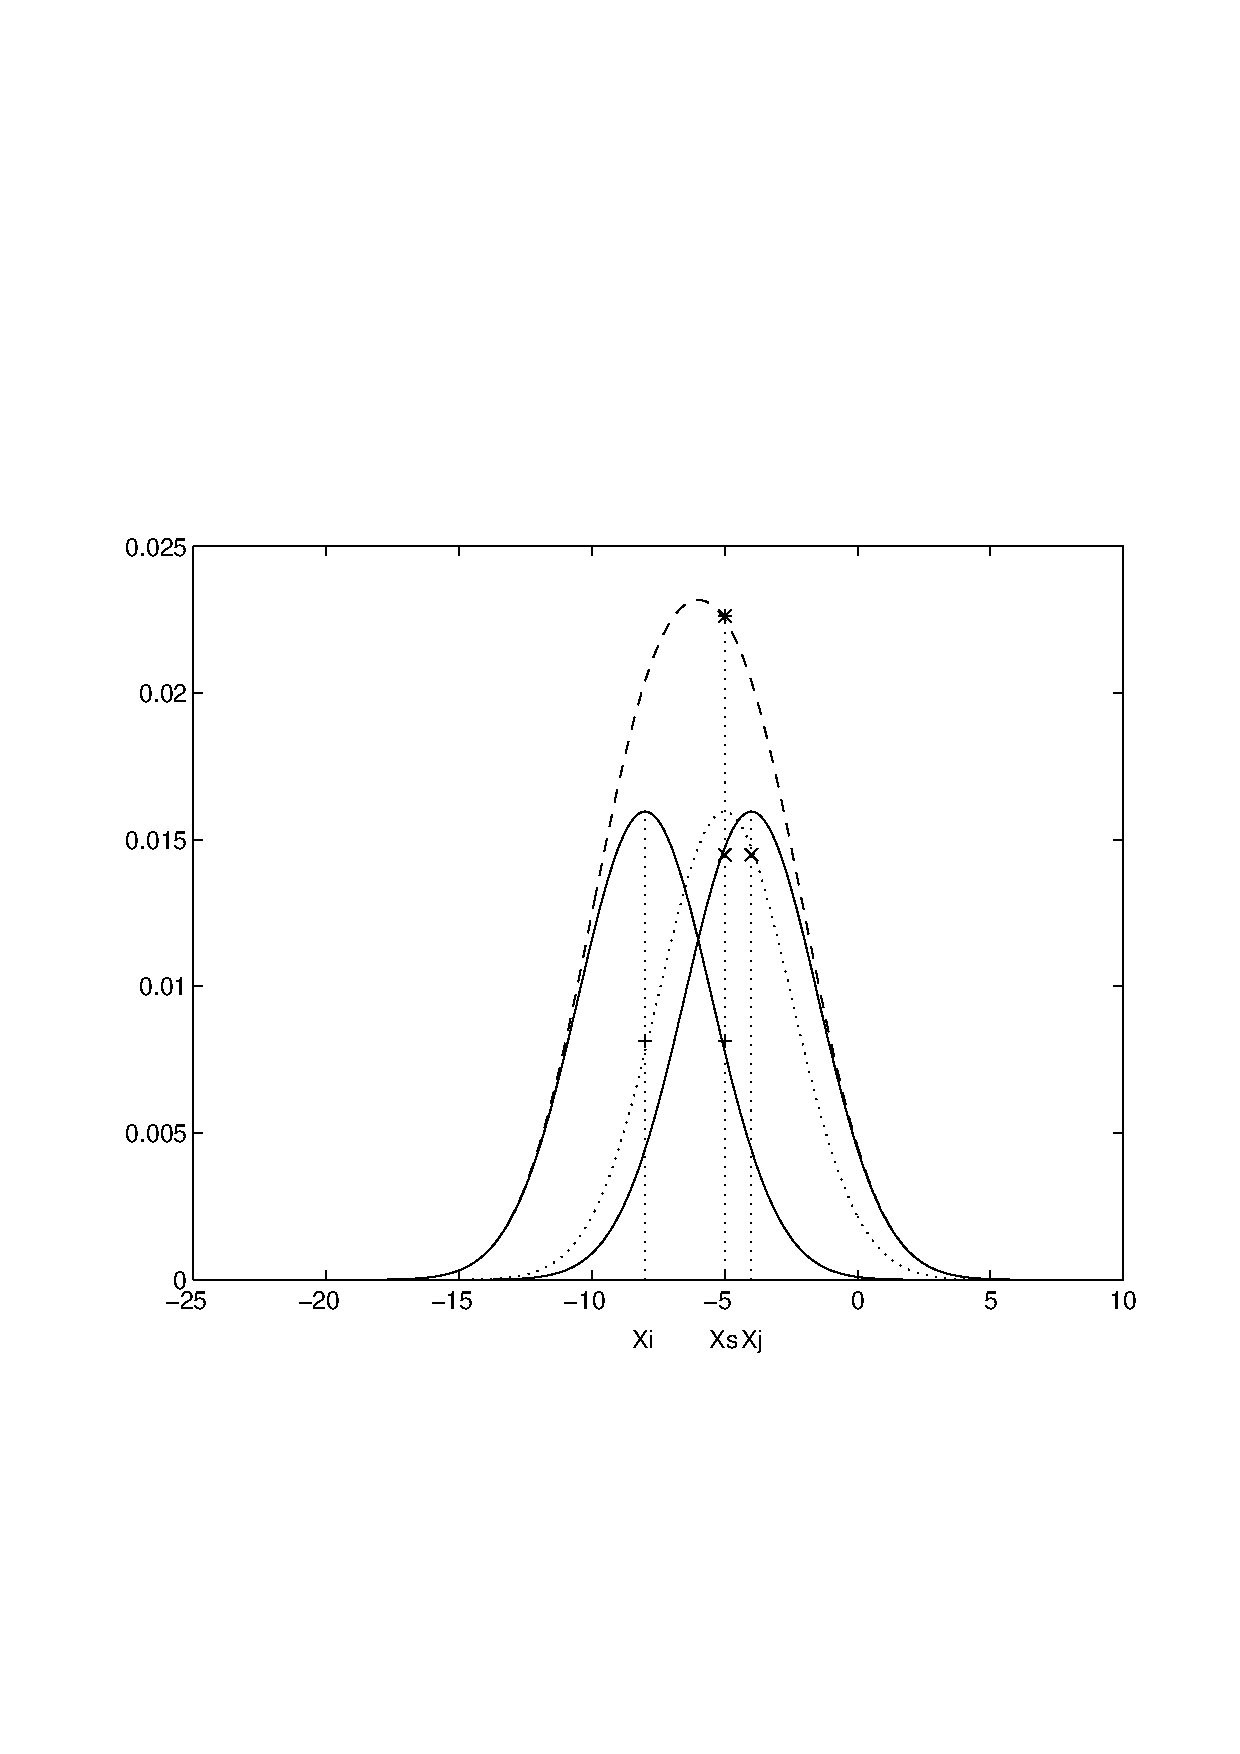
\includegraphics[height=6.2cm]{eijkel2}
%\caption{One kernel at $x_s$ (\emph{dotted kernel}) or two kernels at
%$x_i$ and $x_j$ (\textit{left and right}) lead to the same summed estimate
%at $x_s$. This shows a figure consisting of different types of
%lines. Elements of the figure described in the caption should be set in
%italics, in parentheses, as shown in this sample caption.}
%\label{fig:example}
%\end{figure}
%
%Please define figures (and tables) as floating objects. Please avoid
%using optional location parameters like ``\verb+[h]+" for ``here".
%
%\paragraph{Remark 1.}
%
%In the printed volumes, illustrations are generally black and white
%(halftones), and only in exceptional cases, and if the author is
%prepared to cover the extra cost for color reproduction, are colored
%pictures accepted. Colored pictures are welcome in the electronic
%version free of charge. If you send colored figures that are to be
%printed in black and white, please make sure that they really are
%legible in black and white. Some colors as well as the contrast of
%converted colors show up very poorly when printed in black and white.
%
%\subsection{Formulas}
%
%Displayed equations or formulas are centered and set on a separate
%line (with an extra line or halfline space above and below). Displayed
%expressions should be numbered for reference. The numbers should be
%consecutive within each section or within the contribution,
%with numbers enclosed in parentheses and set on the right margin --
%which is the default if you use the \emph{equation} environment, e.g.,
%\begin{equation}
%  \psi (u) = \int_{o}^{T} \left[\frac{1}{2}
%  \left(\Lambda_{o}^{-1} u,u\right) + N^{\ast} (-u)\right] dt \;  .
%\end{equation}
%
%Equations should be punctuated in the same way as ordinary
%text but with a small space before the end punctuation mark.
%
%\subsection{Footnotes}
%
%The superscript numeral used to refer to a footnote appears in the text
%either directly after the word to be discussed or -in relation to a
%phrase or a sentence -following the punctuation sign (comma,
%semicolon, or period). Footnotes should appear at the bottom of
%the
%normal text area, with a line of about 2~cm set
%immediately above them.\footnote{The footnote numeral is set flush left
%and the text follows with the usual word spacing.}
%
%\subsection{Program Code}
%
%Program listings or program commands in the text are normally set in
%typewriter font, e.g., CMTT10 or Courier.
%
%\medskip
%
%\noindent
%{\it Example of a Computer Program}
%\begin{verbatim}
%program Inflation (Output)
%  {Assuming annual inflation rates of 7%, 8%, and 10%,...
%   years};
%   const
%     MaxYears = 10;
%   var
%     Year: 0..MaxYears;
%     Factor1, Factor2, Factor3: Real;
%   begin
%     Year := 0;
%     Factor1 := 1.0; Factor2 := 1.0; Factor3 := 1.0;
%     WriteLn('Year  7% 8% 10%'); WriteLn;
%     repeat
%       Year := Year + 1;
%       Factor1 := Factor1 * 1.07;
%       Factor2 := Factor2 * 1.08;
%       Factor3 := Factor3 * 1.10;
%       WriteLn(Year:5,Factor1:7:3,Factor2:7:3,Factor3:7:3)
%     until Year = MaxYears
%end.
%\end{verbatim}
%
%\noindent
%{\small (Example from Jensen K., Wirth N. (1991) Pascal user manual and
%report. Springer, New York)}
%
%\subsection{Citations}
%
%For citations in the text please use
%square brackets and consecutive numbers: \cite{jour}, \cite{lncschap},
%\cite{proceeding1} -provided automatically
%by \LaTeX 's \verb|\cite| \dots\verb|\bibitem| mechanism.
%
%\subsection{Page Numbering and Running Heads}
%
%There is no need to include page numbers. If your paper title is too
%long to serve as a running head, it will be shortened. Your suggestion
%as to how to shorten it would be most welcome.
%
%\section{LNCS Online}
%
%The online version of the volume will be available in LNCS Online.
%Members of institutes subscribing to the Lecture Notes in Computer
%Science series have access to all the pdfs of all the online
%publications. Non-subscribers can only read as far as the abstracts. If
%they try to go beyond this point, they are automatically asked, whether
%they would like to order the pdf, and are given instructions as to how
%to do so.
%
%Please note that, if your email address is given in your paper,
%it will also be included in the meta data of the online version.
%
%\section{BibTeX Entries}
%
%The correct BibTeX entries for the Lecture Notes in Computer Science
%volumes can be found at the following Website shortly after the
%publication of the book:
%\url{http://www.informatik.uni-trier.de/~ley/db/journals/lncs.html}
%
%\subsubsection*{Acknowledgments.} The heading should be treated as a
%subsubsection heading and should not be assigned a number.
%
%\section{The References Section}\label{references}
%
%In order to permit cross referencing within LNCS-Online, and eventually
%between different publishers and their online databases, LNCS will,
%from now on, be standardizing the format of the references. This new
%feature will increase the visibility of publications and facilitate
%academic research considerably. Please base your references on the
%examples below. References that don't adhere to this style will be
%reformatted by Springer. You should therefore check your references
%thoroughly when you receive the final pdf of your paper.
%The reference section must be complete. You may not omit references.
%Instructions as to where to find a fuller version of the references are
%not permissible.
%
%We only accept references written using the latin alphabet. If the title
%of the book you are referring to is in Russian or Chinese, then please write
%(in Russian) or (in Chinese) at the end of the transcript or translation
%of the title.
%
%The following section shows a sample reference list with entries for
%journal articles \cite{jour}, an LNCS chapter \cite{lncschap}, a book
%\cite{book}, proceedings without editors \cite{proceeding1} and
%\cite{proceeding2}, as well as a URL \cite{url}.
%Please note that proceedings published in LNCS are not cited with their
%full titles, but with their acronyms!
%
%\begin{thebibliography}{4}
%
%\bibitem{jour} Smith, T.F., Waterman, M.S.: Identification of Common Molecular
%Subsequences. J. Mol. Biol. 147, 195--197 (1981)
%
%\bibitem{lncschap} May, P., Ehrlich, H.C., Steinke, T.: ZIB Structure Prediction Pipeline:
%Composing a Complex Biological Workflow through Web Services. In: Nagel,
%W.E., Walter, W.V., Lehner, W. (eds.) Euro-Par 2006. LNCS, vol. 4128,
%pp. 1148--1158. Springer, Heidelberg (2006)
%
%\bibitem{book} Foster, I., Kesselman, C.: The Grid: Blueprint for a New Computing
%Infrastructure. Morgan Kaufmann, San Francisco (1999)
%
%\bibitem{proceeding1} Czajkowski, K., Fitzgerald, S., Foster, I., Kesselman, C.: Grid
%Information Services for Distributed Resource Sharing. In: 10th IEEE
%International Symposium on High Performance Distributed Computing, pp.
%181--184. IEEE Press, New York (2001)
%
%\bibitem{proceeding2} Foster, I., Kesselman, C., Nick, J., Tuecke, S.: The Physiology of the
%Grid: an Open Grid Services Architecture for Distributed Systems
%Integration. Technical report, Global Grid Forum (2002)
%
%\bibitem{url} National Center for Biotechnology Information, \url{http://www.ncbi.nlm.nih.gov}
%
%\end{thebibliography}
%
%
%\section*{Appendix: Springer-Author Discount}
%
%LNCS authors are entitled to a 33.3\% discount off all Springer
%publications. Before placing an order, the author should send an email, 
%giving full details of his or her Springer publication,
%to \url{orders-HD-individuals@springer.com} to obtain a so-called token. This token is a
%number, which must be entered when placing an order via the Internet, in
%order to obtain the discount.
%
%\section{Checklist of Items to be Sent to Volume Editors}
%Here is a checklist of everything the volume editor requires from you:
%
%
%\begin{itemize}
%\settowidth{\leftmargin}{{\Large$\square$}}\advance\leftmargin\labelsep
%\itemsep8pt\relax
%\renewcommand\labelitemi{{\lower1.5pt\hbox{\Large$\square$}}}
%
%\item The final \LaTeX{} source files
%\item A final PDF file
%\item A copyright form, signed by one author on behalf of all of the
%authors of the paper.
%\item A readme giving the name and email address of the
%corresponding author.
%\end{itemize}

